%\subsubsection{Hubo2 Plus}
The Hubo2 Plus series robot is a 130 $cm$ (4' 3'') tall, 42 $kg$ (93 $lb$) full-size humanoid commonly refereed to as Hubo.  
The Hubo series was designed and constructed by Prof Jun-Ho Oh at the Hubo Lab in the Korean Advanced Institute of Science and Technology (KAIST) in Daejeon, South Korea \cite{1573587}.
Hubo has 2 arms, 2 legs and a head making it anthropomorphic to a human.
It contains 6 degrees of freedom (DOF) in each leg, 6 in each arm, 5 in each hand, 3 in the neck, and 1 in the waist; all totaling 38 DOF.
All joints of the major joints are high gain PID position controlled with the exception of the fingers.
The fingers are open-loop PWM controlled.
The sensing capability consists of a three axis force-torque (FT) sensor on each leg between the end of the ankle and the foot as well as between the arm where it connects to the hand.
Additionally it has an inertial measurement unit (IMU) at the center of mass and accelerometers on each foot.
The reference commands for all of the joints are sent from the primary control computer (x86) to the individual motor controllers via two Controller Area Network (CAN) buses.
There are currently eight Hubo's functioning in the United States as of December 2012.
Jaemi Hubo is the oldest of the Hubos in America and has been at the Drexel Autonomous Systems Lab\footnote{Drexel Autonomous Systems Lab: http://dasl.mem.drexel.edu/} (DASL) since 2008 \cite{jaemiHuboSRM}.
Fig.~\ref{fig:hubo} shows the major dimensions of Hubo.
Table~\ref{table:huboSensors} shows the other attributes of the Hubo.
%(휴보) 

A full-scale safe testing environment designed for experiments with Jaemi Hubo was created using DASL's Systems Integrated Sensor Test Rig (SISTR)~\cite{5686325}.  
Additionally all algorithms are able to be tested on miniature and virtual versions of Jaemi Hubo prior to testing on the full-size humanoid through the creation of a surrogate testing platform for humanoids~\cite{5379582}.

\begin{figure}[thpb]
  \centering
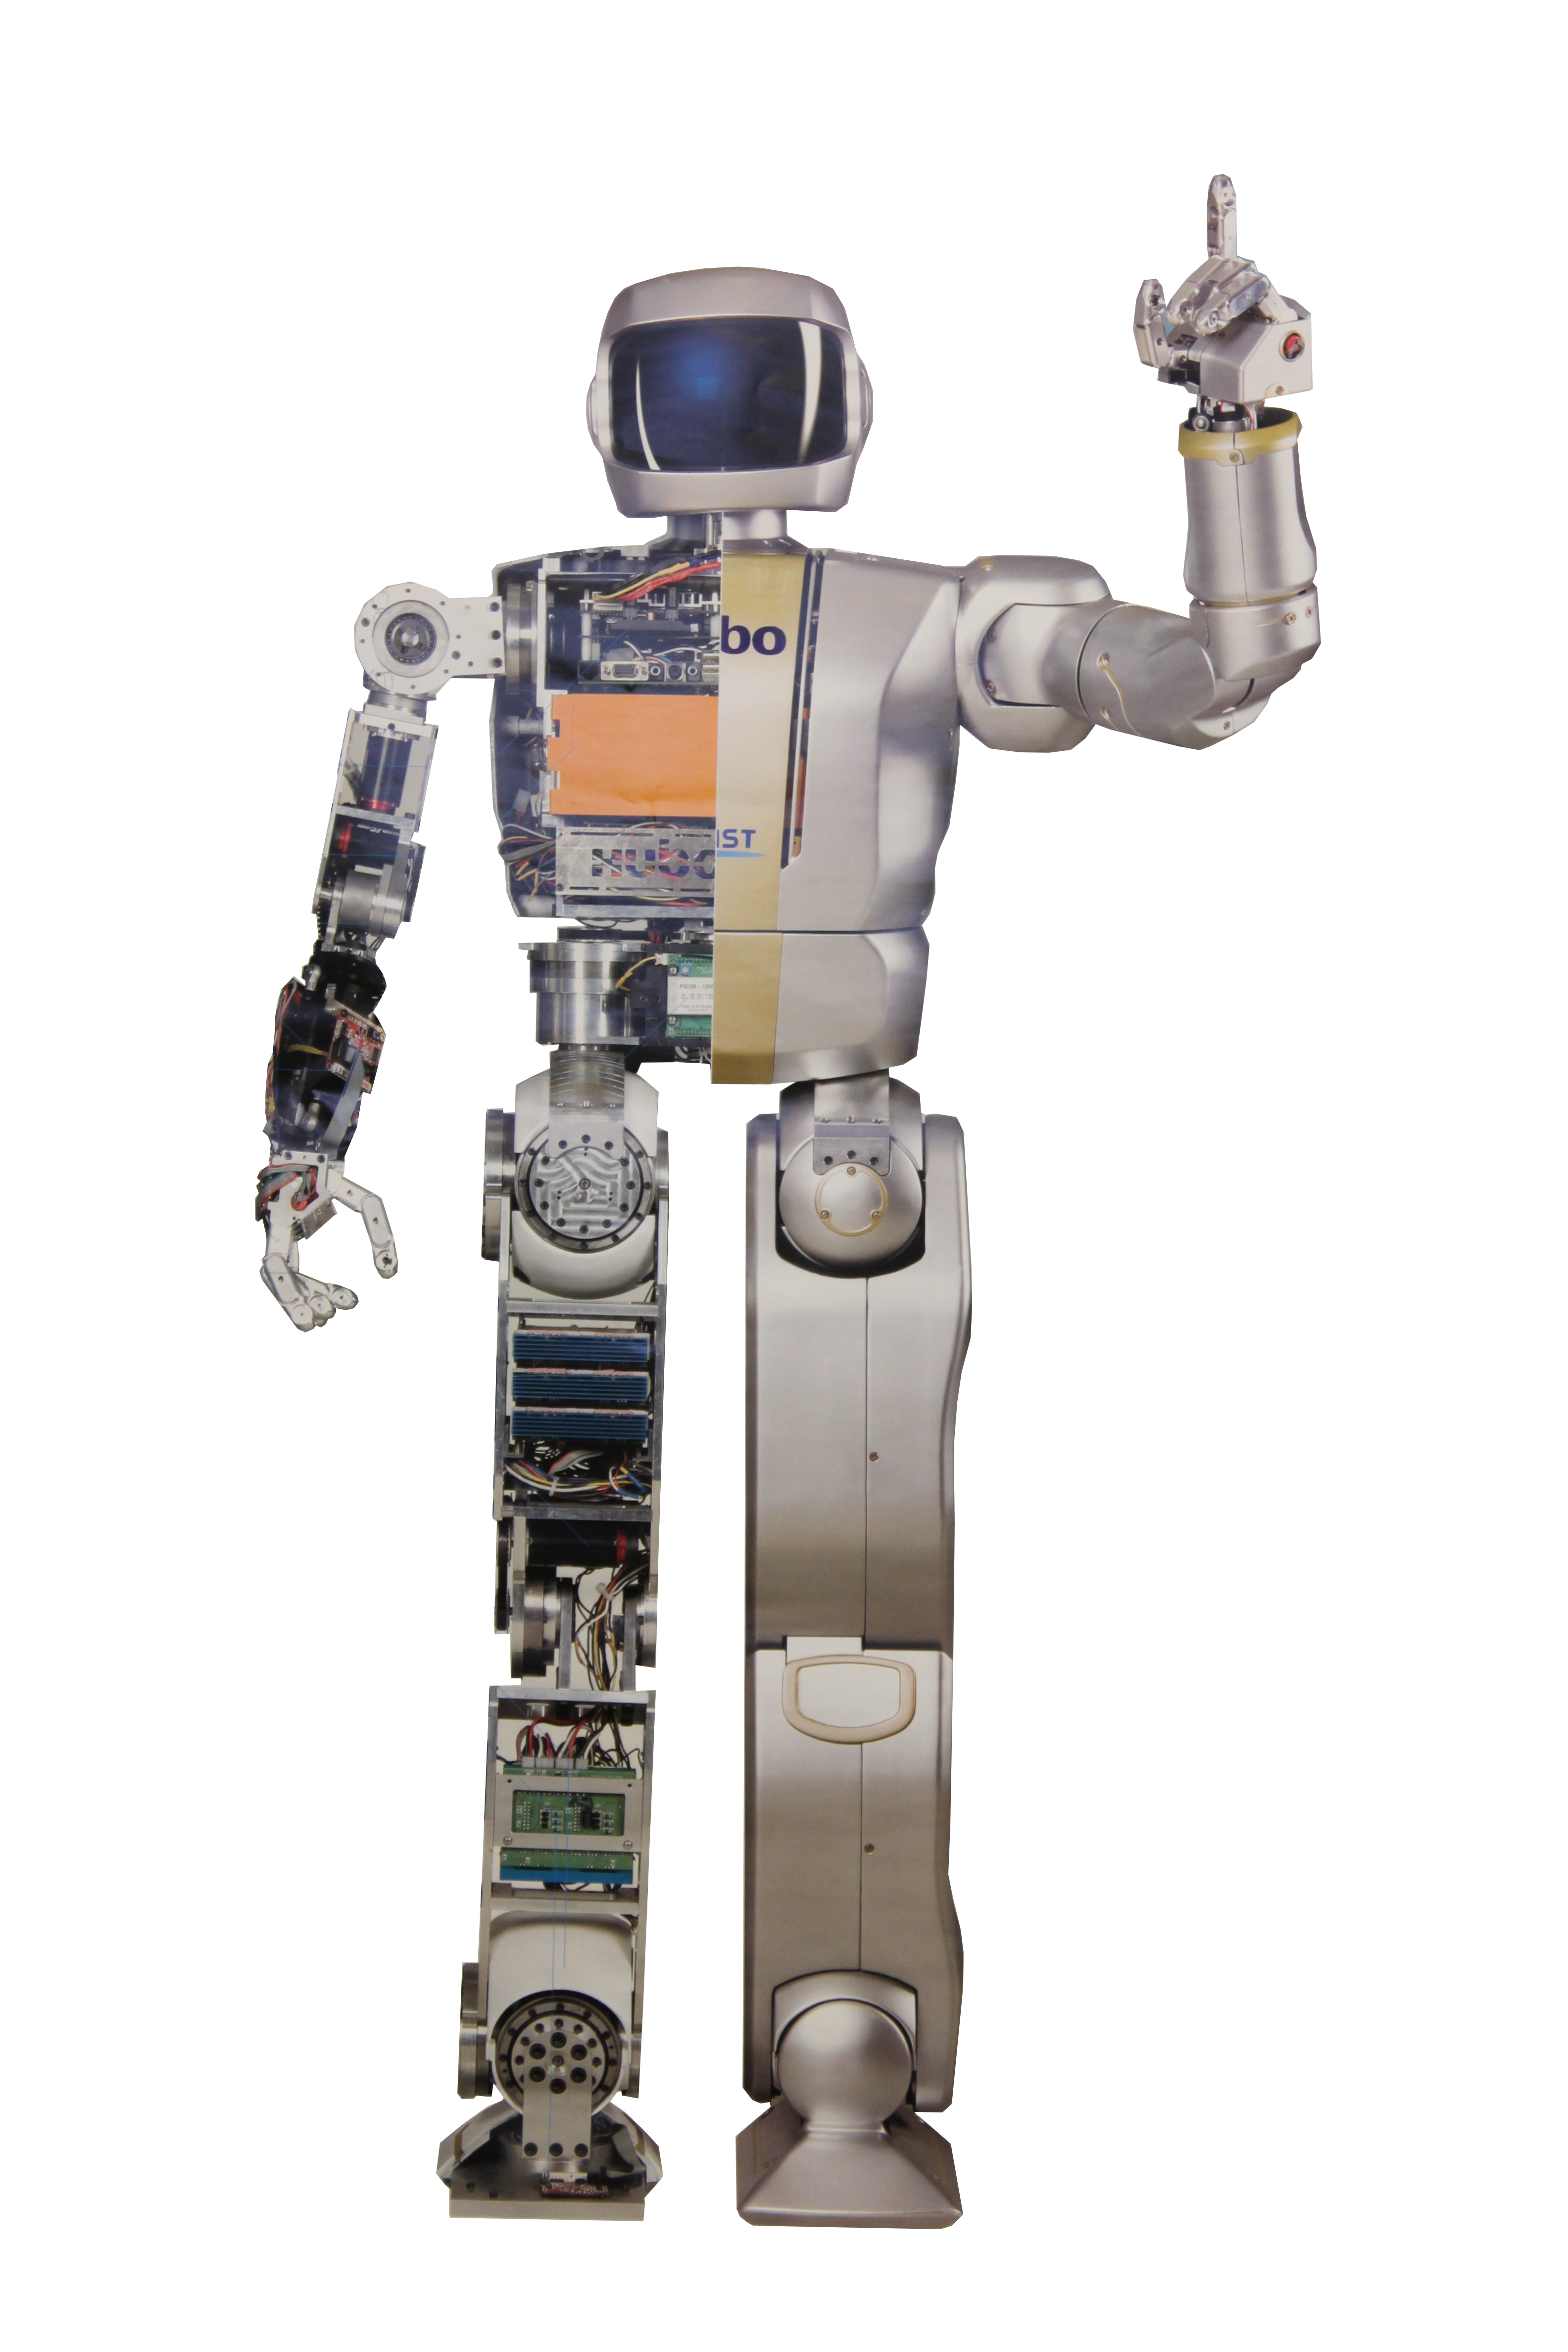
\includegraphics[width=0.37\columnwidth]{./background/pix/huboReal.png}\includegraphics[width=0.63\columnwidth]{./pix/huboSkel.pdf}
  \caption{Hubo2 Plus platform: 40 DOF, 130 $cm$ tall full-size humanoid robot weighing 37 $kg$.}
  \label{fig:hubo}
\end{figure}


\begin{table}
\centering
\caption{Hubo2 Plus (Hubo) Platform Specifications}
\begin{tabular}{| l || l |}
\hline
Height      		& $130~cm$			\\
\hline
Weight			& $37~kg$			\\
\hline
DOF			& 40				\\
\hline
Joint Control Type	& High-Gain PID Position	\\
\hline
Computer		& $1.6~Ghz$ Atom		\\
			& $1~Gb$ DDR3 RAM		\\
\hline
Operating System	& Debian Linux			\\
			& Windows			\\
\hline
Battery			& $54V$ $7.5~Ah$ $40C$ LiPo	\\
\hline
Sensors			& 1x 4 Axis IMU			\\
			& 4x 3 Axis Force Torque	\\
			& 2x 2 Axis Tilt		\\
\hline
Vision			& Stereo			\\
			& Monocular			\\
			& RGBD				\\
\hline
\end{tabular}
\label{table:huboSensors}
\end{table}



